\documentclass[25pt, a0paper, portrait]{tikzposter}
\newcommand{\posterfigure}[2]{%
	\begin{center}
		\begin{tikzpicture}
			% Draws a flat background placeholder box
			\fill[CanvaNavy!10] (-10, -5) rectangle (10, 5);
			% Safely overlays the image and text box without bounding box violations
			\node[text width=18cm, align=center] at (0,0) {
				% Un-comment the line below when your image files are ready in the folder path:
				 \includegraphics[width=14cm]{#1} \\ \vspace{0.5cm}
				\Large \textbf{#2}
			};
		\end{tikzpicture}
	\end{center}
}
% MACRO 2: Paired Side-by-Side Figures (Fixes stacking issue)
% Usage: \posterpairedfigures{img1}{cap1}{img2}{cap2}
\newcommand{\posterpairedfigures}[4]{%
	\begin{center}
		\begin{tikzpicture}
			% Left Box Background and Text
			\fill[CanvaNavy!10] (-9.5, -5) rectangle (-0.5, 5);
			\node[text width=8.5cm, align=center] at (-5,0) {
				\includegraphics[width=8cm]{#1} \\ \vspace{0.5cm}
				\Large \textbf{#2}
			};
			
			% Right Box Background and Text
			\fill[CanvaNavy!10] (0.5, -5) rectangle (9.5, 5);
			\node[text width=8.5cm, align=center] at (5,0) {
				 \includegraphics[width=8cm]{#3} \\ \vspace{0.5cm}
				\Large \textbf{#4}
			};
		\end{tikzpicture}
	\end{center}
}

% ==========================================
% 1. TYPOGRAPHY & ENCODING
% ==========================================
\usepackage[utf8]{inputenc}
\usepackage[T1]{fontenc}
\usepackage[defaultfam]{montserrat} % Classically modern, wide geometric sans
\usepackage{graphicx} % Required for inserting placeholder images
\renewcommand{\familydefault}{\sfdefault}

% ==========================================
% 2. CANVA-STYLE FLAT COLOR PALETTE
% ==========================================
\definecolor{CanvaNavy}{HTML}{1E2B3C}
\definecolor{CanvaOrange}{HTML}{EF8354}
\definecolor{CanvaSand}{HTML}{F4F1DE}
\definecolor{CanvaTeal}{HTML}{457B9D}
\definecolor{CanvaWhite}{HTML}{FFFFFF}

% Pre-mix the color to avoid tikzposter parsing errors
\colorlet{LightTeal}{CanvaTeal!10}

% Override tikzposter defaults to remove gradients and shadows
\tikzposterlatexaffectionproofoff % Removes the tikzposter watermark

\definecolorstyle{FlatColorStyle}{
	\colorlet{colorOne}{CanvaNavy}
	\colorlet{colorTwo}{CanvaSand}
	\colorlet{colorThree}{CanvaTeal}
}{
	% Background Colors
	\colorlet{backgroundcolor}{CanvaSand}
	\colorlet{framecolor}{CanvaSand}
	% Title Colors
	\colorlet{titlebgcolor}{CanvaNavy}
	\colorlet{titlefgcolor}{CanvaWhite}
	% Block Colors
	\colorlet{blocktitlebgcolor}{CanvaWhite}
	\colorlet{blocktitlefgcolor}{CanvaNavy}
	\colorlet{blockbodybgcolor}{CanvaWhite}
	\colorlet{blockbodyfgcolor}{black}
}

\definetitlestyle{FlatTitle}{
	width=\paperwidth, linewidth=0pt, innersep=2cm,
	titletotopverticalspace=0mm, titletoblockverticalspace=20mm
}{
	\begin{scope}[line width=\titlelinewidth]
		\draw[color=blocktitlebgcolor, fill=titlebgcolor]
		(\titleposleft,\titleposbottom) rectangle (\titleposright,\titlepostop);
	\end{scope}
}

\defineblockstyle{FlatBlock}{
	titlewidthscale=1, bodywidthscale=1, titleleft,
	titleoffsetx=0pt, titleoffsety=0pt, bodyoffsetx=0pt, bodyoffsety=0pt,
	bodyverticalshift=0pt, roundedcorners=0, linewidth=0pt,
	titleinnersep=1cm, bodyinnersep=1cm
}{
	\begin{scope}[line width=\blocklinewidth]
		\ifBlockHasTitle
		% Draw flat white background for the whole block
		\draw[fill=blockbodybgcolor, draw=none]
		(blockbody.south west) rectangle (blocktitle.north east);
		% Add a thick accent line on the left side of the title
		\draw[color=CanvaOrange, line width=10pt] 
		(blocktitle.south west) -- (blocktitle.north west);
		\else
		\draw[fill=blockbodybgcolor, draw=none]
		(blockbody.south west) rectangle (blockbody.north east);
		\fi
	\end{scope}
}

\usecolorstyle{FlatColorStyle}
\usetitlestyle{FlatTitle}
\useblockstyle{FlatBlock}
\usebackgroundstyle{Empty}

% ==========================================
% 3. TITLE & AUTHOR INFO
% ==========================================
\title{
	\parbox{\linewidth}{\centering 
		% The Main Title: Ultra bold, all caps
		\textbf{\MakeUppercase{Disk-Stacking and Fibonacci spirals}} \\ 
		\vspace{0.8cm} 
		% The Subtitle
		\Large \textcolor{CanvaSand}{A new old paradigm for morphogenesis}
	}
}

\author{
	\vspace{0.5cm} 
	\Large \textbf{Jonathan Swinton} \quad \textcolor{CanvaOrange}{|} \quad \normalsize jonathan@swintons.net
}

\begin{document}
	
	\maketitle
	
	\begin{columns}
		
		% ------------------------------------------
		% LEFT COLUMN
		% ------------------------------------------
		\column{0.49}
		
		\block{An open problem}{
			Most mathematicians know that Fibonacci spirals can be found in plants.
		Fewer know this topic offers rich open mathematical questions \textit{and} generates hypotheses testable by modern molecular biology. 
			
		
		}
		
		\block{An old observation}{	
		
			\posterfigure{./Figures/sunflowers(12)-55.jpg}{Find the Fibonacci number!}
		}
		
		
		\block{Cylindrical lattices have two parameters \& display parastichy numbers}{
	\posterpairedfigures{./Figures/Txb0403Coordinates}{Rise and divergence}
			{./Figures/Txb0403Coordinates}{Rise and divergence}
	
			
		
		}
		
		
		\block{Disk-Stacking Methodology}{
			Disk-stacking models were first introduced by Schwendener in the 1870s as an exploration of organ placement in plants [cite: 126]. The deterministic model is entirely defined by the function $r_{i}$, which gives the radius of the $i$th disk based on the height of the most recently placed disk [cite: 132, 133].
			
			\vspace{0.5cm}
			\begin{itemize}
				\item \textbf{Control Parameter:} The slope $r^{\prime}$ is used as the control parameter, corresponding to the speed at which the disk size changes [cite: 134].
				\item \textbf{Stochasticity:} Noise is introduced by multiplying the radius by a scaling factor drawn from a uniform distribution of $[1-\sigma,1+\sigma]$ [cite: 135].
				\item \textbf{Transitions:} Parastichy numbers in stacked-disk models change at $\gamma$ and A dislocations [cite: 163]. Each jump corresponds to a $\gamma$ dislocation of the parastichy lines, while A dislocations correspond to a decrease in the count [cite: 172, 173].
			\end{itemize}
		}
		
		% ------------------------------------------
		% RIGHT COLUMN
		% ------------------------------------------
		\column{0.49}
		
		\block{Observational Data \& Results}{
			The reference dataset is taken from the MOSI Turing's Sunflower's project collection [cite: 210]. 
			
			\vspace{0.5cm}
			\begin{itemize}
				\item There was a strong but not complete preponderance of Fibonacci counts [cite: 212].
				\item Excluding Fibonacci counts, the next commonest parastichy count was one less than a Fibonacci number (e.g., 33, 54, or 88) [cite: 213].
				\item This was followed by Lucas numbers (29, 47, or 76) and double-Fibonacci numbers (42, 68) [cite: 215].
			\end{itemize}
			
			\vspace{1cm}
			\begin{center}
				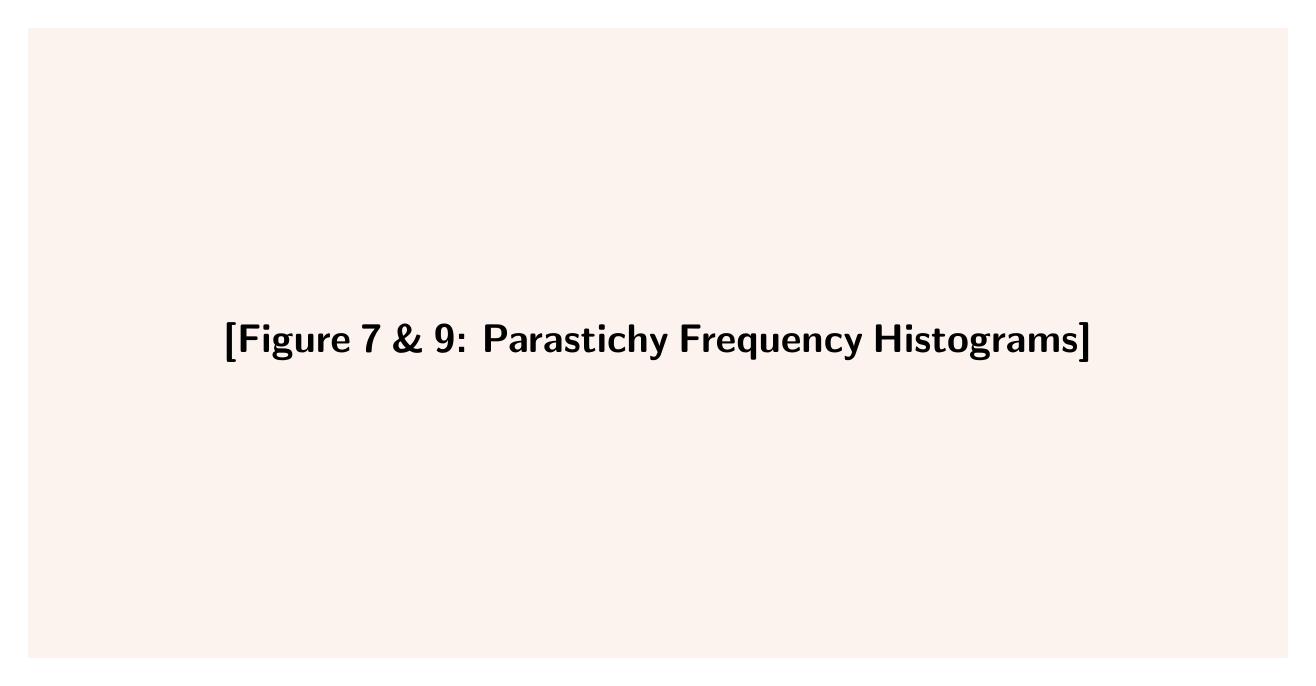
\begin{tikzpicture}
					% This draws a flat placeholder box
					\fill[CanvaOrange!10] (-8, -4) rectangle (8, 4);
					\node[text width=14cm, align=center] at (0,0) {
						\Large \textbf{[Figure 7 \& 9: Parastichy Frequency Histograms]}
					};
				\end{tikzpicture}
			\end{center}
			
			\vspace{1cm}
			Slow change rates support Fibonacci transitions [cite: 219]. However, rapid transitions promote near-Fibonacci counts, while noise promotes columnar structures [cite: 380]. Furthermore, double-Fibonacci and Lucas numbers emerge at large scales near the critical $r^{\prime}$ and are promoted by noise [cite: 433].
		}
		
		\block{This work adds}{
			The dynamics of slowly changing stacked-disk models naturally generate well-ordered lattice-like patterns with Fibonacci structure, providing a rationale for Turing's 'hypothesis of geometrical phyllotaxis' [cite: 455]. 
			
			For faster rates of disk change, different parastichy counts emerge in ways highly compatible with observed data [cite: 456]. Ultimately, there is 'no gene for the number 55'; the observed structural motifs of phyllotaxis can only be understood in the light of a mathematical understanding of pattern dynamics [cite: 500].
			
			\vspace{0.5cm}
			\coloredbox[width=0.9\linewidth, bgcolor=LightTeal, fgcolor=black, framecolor=LightTeal]{
				\textbf{Key Finding:} The models account for a predominance of Fibonacci counts, while also explaining a smaller but detectable frequency of Lucas numbers, double Fibonacci numbers, and pairs of roughly equal but non-Fibonacci counts in a 'columnar' structure [cite: 5].
			}
		}
		
		\block{TL;DR}{
			Disk stacking models are mathematically intriguing, computationally tractable, and have application to an old but still open biological problem: why do plants have Fibonacci numbers? 
		}
	\end{columns}
	
\end{document}
